\documentclass{article}
\usepackage[utf8]{inputenc}
\usepackage{amsmath}
\usepackage{amssymb}
\usepackage{graphicx}

\newcommand\tr{\mathsf{T}}
\newcommand\hr{\mathsf{H}}

\begin{document}
\section*{Cholesky and QR decomposition}
\subsection*{2-4.a}
We are tasked with showing that for every matrix $\mathbf{A} \in \mathbb{R}^{m,n}$ with $\text{rank}\left(\mathbf{A}\right) = n$ the product matrix $\mathbf{A}^{\tr}\mathbf{A}$ admits a Cholesky decomposition. Let us look at the lemma that introduces the Cholesky decomposition in the lecture document.

\begin{figure}[!hbt]
    \centering
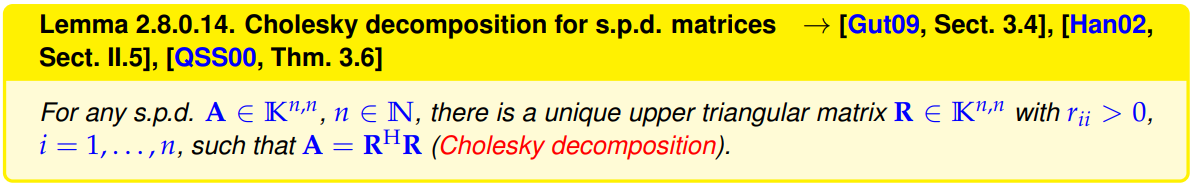
\includegraphics[width=1.0\linewidth]{CholeskyDecomposition.png}
\end{figure}

\noindent We thus want to show that for any matrix $\mathbf{A}$ with $\text{rank}\left(\mathbf{A}\right) = n$ that  $\mathbf{A}^{\tr}\mathbf{A}$ is symmetric positive definite. Let us first show that it is symmetric.

\begin{equation*}
    \left(\mathbf{A}^{\tr}\mathbf{A}\right)^{\tr} = \mathbf{A}^{\tr}\left(\mathbf{A}^{\tr}\right)^{\tr} = \mathbf{A}^{\tr}\mathbf{A}
\end{equation*}
Now let us prove that $\mathbf{A}^{\tr}\mathbf{A}$ is positive definite. We now know because $\mathbf{A}$ has full rank and because it is a square matrix that $\mathbf{A}^{\tr}$ must have full rank as well (column-rank $=$ row-rank). We can thus apply the following Lemma
\begin{figure}[!hbt]
    \centering
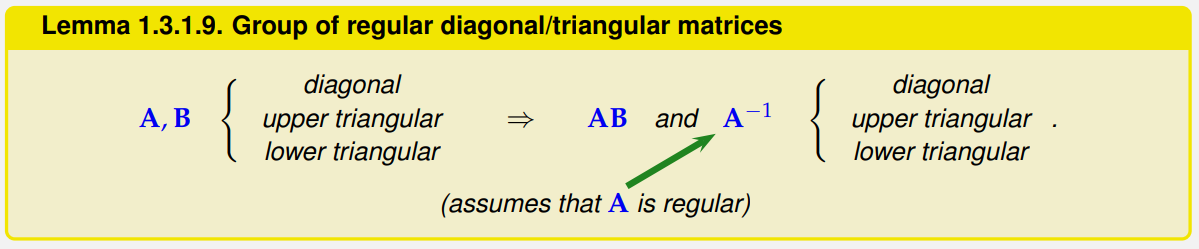
\includegraphics[width=1.0\linewidth]{ProductRegularity.png}
\end{figure}
this tells us that $\mathbf{A}^{\tr}\mathbf{A}$ has full rank and thus we have $\text{ker}\left(\mathbf{A}^{\tr}\mathbf{A}\right) = \left\{0\right\}$. Thus for any $\mathbf{v}\neq \mathbf{0}$ we have $\mathbf{A}\mathbf{v} \neq \mathbf{0}$. We also have
\begin{equation*}
    \mathbf{v}^{\tr}\left(\mathbf{A}^{\tr}\mathbf{A}\right)\mathbf{v} = \left(\mathbf{v}^{\tr}\mathbf{A}^{\tr}\right)\left(\mathbf{A}\mathbf{v}\right) = \left(\mathbf{A}\mathbf{v}\right)^{\tr}\left(\mathbf{A}\mathbf{v}\right) = \left\lVert \mathbf{A}\mathbf{v}\right\rVert_{2}^{2} \geq 0
\end{equation*}
For $\mathbf{v}\neq \mathbf{0}$ we have $\left\lVert \mathbf{A}\mathbf{v}\right\rVert_{2}^{2} > 0$ though and thus 
 > 0$\mathbf{v}^{\tr}\left(\mathbf{A}^{\tr}\mathbf{A}\right)\mathbf{v}
 > 0$ and for $\mathbf{v} = \mathbf{0}$ we have $\mathbf{v}^{\tr}\left(\mathbf{A}^{\tr}\mathbf{A}\right)\mathbf{v}
 = 0$, which is exactly the definition of being positive definite. Hence we can conclude that  $\mathbf{A}^{\tr}\mathbf{A}$ is positive definite and by Lemma 2.8.0.14 it thus has a Cholesky decomposition.

 \subsection*{2-4.b}
 We are given two Eigen functions and are tasked to prove that they produce the same output matrices $\mathbf{Q}$ and $\mathbf{R}$ for the same input matrix $\mathbf{A}$ when disregarding roundoff errors. Let us first discuss some things, firstly we know that \verb|HouseholderQR| does not employ permutations of the given input matrix $\mathbf{A}$, which can be taken from the hint or from the Eigen documentation (\verb|ColPivHouseholderQR| and \verb|FullPivHouseholderQR| do us pivoting) and secondly both functions only compute the economical QR-decomposition, as the hint tells us. First let us look at the code segment that uses the Cholesky-decomposition to compute the QR-decomposition

 \begin{figure}[!hbt]
    \centering
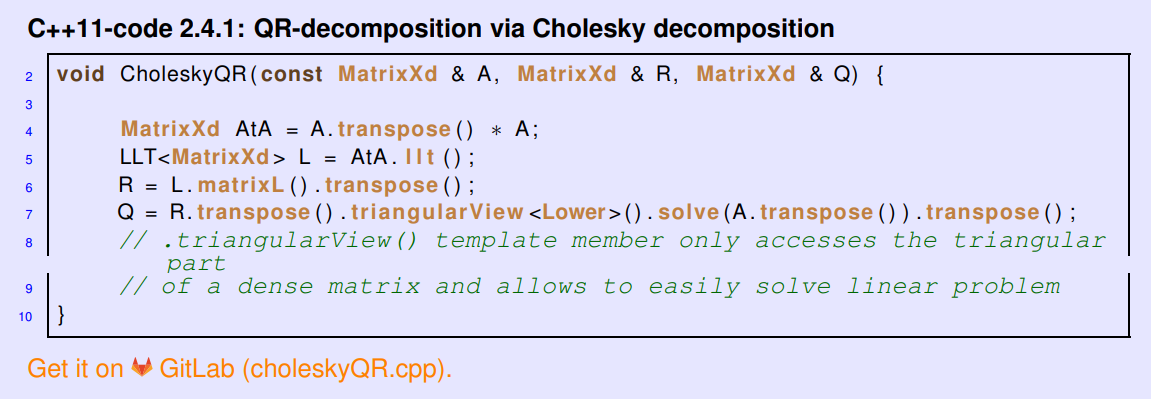
\includegraphics[width=1.0\linewidth]{QRDecompCholesky.png}
\end{figure}

\noindent The first line computes $\mathbf{A}^{\tr}\mathbf{A}$ from $\mathbf{A}$. The second line computes a Cholesky-decomposition (given by \verb|Eigen::LLT|) of $\mathbf{A}^{\tr}\mathbf{A}$, we can use the Cholesky-decomposition given to us by \verb|Eigen::LLT| here, because $\mathbf{A}$ is positive definite, were $\mathbf{A}$ positive semi-definite we would have to use \verb|Eigen::LDLT| instead. It is important to state that the Eigen function computes the same Cholesky-decomposition as in the definition but instead of interpreting it as $\mathbf{R}^{\hr}\mathbf{R}$ for some upper triangular matrix $\mathbf{
R}$ it interpretes it as $\mathbf{L}\mathbf{L}^{\hr}$ for some lower triangular matrix $\mathbf{L}$.  Hence when the code does \verb|R = L.matrixL().transpose()| we do compute $\mathbf{R}$ as above from $\mathbf{L}$ (the Eigen Cholesky factor). We hence denote the Cholseky decomposition of $\mathbf{A}^{\tr}\mathbf{A}$ by
\begin{equation*}
    \mathbf{A}^{\tr}\mathbf{A} = \mathbf{R}^{\tr}\mathbf{R} 
\end{equation*}
we then define $\mathbf{Q}$ to have columns being the solution to the linear systems of equations. Let us do this step by step, we are given the code line \\[2mm]
\verb|Q = R.transpose().triangularView<Eigen::Lower>().solve(A.transpose()).transpose()|
\\[1mm]
There is a lot happening here, first we use \verb|triangularView| only to make it possible for Eigen to see the structure and be able to solve the given system by forward substitution. We then also transpose the final solution, which means that the individual system give us the rows of $\mathbf{Q}$, we also see that in general the result of solving (this is pseudocode, we cannot invoke a solver on a simple \verb|Eigen::MatrixXd| object) \\[2mm]
\verb|X = A.solve(B)|
\\[1mm]
is given by
\begin{equation*}
    \mathbf{A}\mathbf{X} = \mathbf{B} \Longleftrightarrow \mathbf{A}^{-1}\mathbf{B}
\end{equation*}
and hence in the above case
\begin{equation*}
    \mathbf{R}^{\tr}\mathbf{Q}^{\tr} = \mathbf{A}^{\tr} \Longleftrightarrow \mathbf{Q}^{\tr} = \left(\mathbf{R}^{\tr}\right)^{-1}\mathbf{A}^{\tr} \Longleftrightarrow \mathbf{Q}^{\tr} = \left(\mathbf{R}^{-1}\right)^{\tr}\mathbf{A}^{\tr}
\end{equation*}
We then transpose the result to give us
\begin{equation*}
    \mathbf{Q} = \left(\left(\mathbf{R}^{-1}\right)^{\tr}\mathbf{A}^{\tr}\right)^{\tr}  = \left(\mathbf{A}^{\tr}\right)^{\tr}\left(\left(\mathbf{R}^{-1}\right)^{\tr}\right)^{\tr} = \mathbf{A}\mathbf{R}^{-1}
\end{equation*}
since we already define the $\mathbf{R}$ we get from the Cholesky- decomposition to be the same as the $\mathbf{R}$ we get in the QR-decomposition, it would be sensible that the above is true, becaue
\begin{equation*}
    \mathbf{Q} = \mathbf{A}\mathbf{R}^{-1} \Longleftrightarrow \mathbf{A} = \mathbf{Q}\mathbf{R}
\end{equation*} 
All that is left to show is that both $\mathbf{R}$ are the same. We do this by first assuming that we are given a QR-decomposition of $\mathbf{A}$ as
\begin{equation*}
    \mathbf{A} = \mathbf{Q}\mathbf{R}
\end{equation*}
from this we get (keep in mind that $\mathbf{Q}$ is orthonormal columns, i.e. $\mathbf{Q}^{\tr}\mathbf{Q} = \mathbf{I}$)
\begin{equation*}
    \mathbf{A}^{\tr}\mathbf{A} = \left(\mathbf{Q}\mathbf{R}\right)^{\tr}\mathbf{Q}\mathbf{R} = \left(\mathbf{R}^{\tr}\mathbf{Q}^{\tr}\right)\mathbf{Q}\mathbf{R} = \mathbf{R}^{\tr}\big(\underbrace{\mathbf{Q}^{\tr}\mathbf{Q}}_{= \mathbf{I}}\big)\mathbf{R} = \mathbf{R}^{\tr}\mathbf{R}
\end{equation*}
and hence we get the Cholesky-decomposition of $\mathbf{A}^{\tr}\mathbf{A}$ from the QR-decomposition of $\mathbf{A}$. On the other hand given a Cholesky-decomposition of $\mathbf{A}^{\tr}\mathbf{A}$ by
\begin{equation*}
    \mathbf{A}^{\tr}\mathbf{A} = \mathbf{R}^{\tr}\mathbf{R}
\end{equation*}
from this we want to construct a matrix with orthogonal columns $\mathbf{
Q}$. We choose as above the matrix $\mathbf{Q} = \mathbf{A}\mathbf{R}^{-1}$, we then use that $\mathbf{A}$ has $\text{rank}\left(\mathbf{A}\right) = n$ and because $\mathbf{R} \in \mathbb{n,n}$ it mus be invertible and we hence can write
\begin{equation*}
    \mathbf{R}^{\tr}\mathbf{R} = \mathbf{A}^{\tr}\mathbf{A} \implies \left(\mathbf{R}^{\tr}\right)^{-1}\left(\mathbf{A}^{\tr}\mathbf{A}\right)\mathbf{R}^{-1} = \mathbf{I} \Longleftrightarrow \underbrace{\left(\mathbf{A}\mathbf{R}^{-1}\right)^{\tr}}_{= \mathbf{Q}^{\tr}}\underbrace{\mathbf{A}\mathbf{R}^{-1}}_{=\mathbf{Q}} = \mathbf{I}
\end{equation*}
and thus $\mathbf{Q} = \mathbf{A}\mathbf{R}^{-1}$ has orthogonal columns and is the $\mathbf{Q}$ factor to $\mathbf{R}$ we were looking for, hence both methods are equivalent.

\subsection*{2-4.c}
We denote by $\mathrm{EPS}$ the machine precision, we are tasked with determining why \verb|CholeskyQR| returns the wrong result for 
\begin{equation*}
    \mathbf{A} = 
    \begin{bmatrix}
    1 & 1 \\
    \frac{1}{2}\mathrm{EPS} & 0 \\
    0 & \frac{1}{2}\mathrm{EPS}
    \end{bmatrix}
\end{equation*}

\pagebreak

\noindent Let us first consider what happens when we compute $\mathbf{A}^{\tr}\mathbf{A}$

\begin{equation*}
    \mathbf{A}^{\tr}\mathbf{A} = \begin{bmatrix}
        1 & \frac{1}{2}\mathrm{EPS} & 0 \\
        1 &  0 & \frac{1}{2}\mathrm{EPS}
    \end{bmatrix} 
    \begin{bmatrix}
    1 & 1 \\
    \frac{1}{2}\mathrm{EPS} & 0 \\
    0 & \frac{1}{2}\mathrm{EPS}
    \end{bmatrix} = \begin{bmatrix}
        1 + \left(\frac{1}{2}\mathrm{EPS}\right)^{2} & 1 \\
        1 & 1 + \left(\frac{1}{2}\mathrm{EPS}\right)^{2}
    \end{bmatrix}
\end{equation*}
We must now remember that because $\frac{1}{2}\mathrm{EPS} < \mathrm{EPS}$ and even more importantly $\mathrm{EPS}$ is the smallest number for which we still have $1 + \mathrm{EPS} > 1$ and $\left(\frac{1}{2}\mathrm{EPS}\right)^{2} < \frac{1}{2}\mathrm{EPS}$, hence we have
\begin{equation*}
    1 + \frac{1}{2}\mathrm{EPS} = 1
\end{equation*}
which leads to
\begin{equation*}
    \mathbf{A}^{\tr}\mathbf{A} = \begin{bmatrix}
        1 & 1 \\
        1 & 1
    \end{bmatrix}
\end{equation*}
this matrix has not full rank and thus its determinant must be zero. This means (because the determinant is the product of the eigenvalues) that at least one of the eigenvalues must be zero. A matrix cannot be positive definite if not all eigenvalue are positive ($> 0$) and hence $\mathbf{A}^{\tr}\mathbf{A}$ is not positive definite and as a result we do not get a Cholesky-decomposition by the lemma above.
\end{document}
